
\subsection{Frame Aggregator}
\label{sec:Frame Aggregator}
The decoded frames are passed into a frame aggregator stage as a first step, which utilizes data aggregation to reduce possible data sparsity of individual frames. 
Data aggregation involves combining multiple consecutive data sets to create a more comprehensive and reliable dataset for processing. This approach increases both useful information and noise, but ultimately enhances the quality of radar point clouds for object detection and tracking stability.
For point clouds from radar sensors, aggregating multiple frames enhances data consistency and density, improving the system’s ability to reconstruct objects and detect motion patterns.

\subsubsection{Single Frame}
Using radar point cloud data from a single frame has inherent limitations, which can lead to incomplete or misleading detections:
\begin{itemize}
    \item A single frame may not capture enough points, leading to failed detections or incomplete object reconstruction.
    \item Limited point data can cause objects to appear fragmented or indistinguishable from noise.
\end{itemize}

\begin{figure}[!htbp]
    \centering
    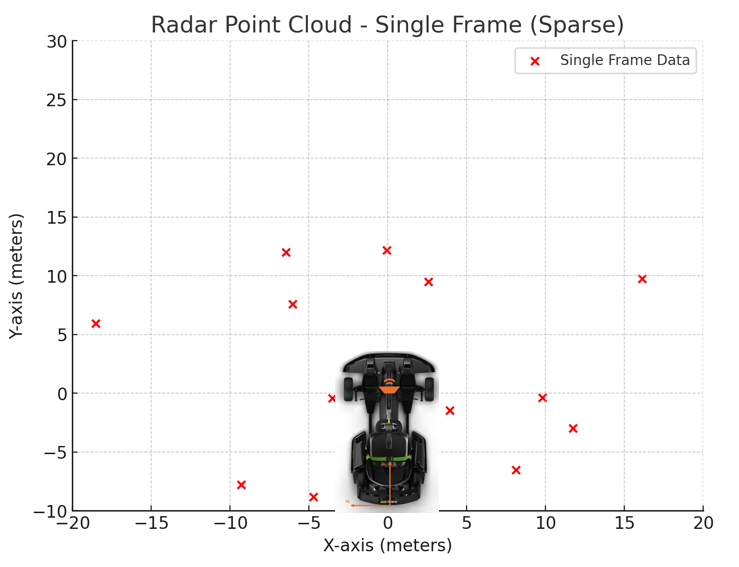
\includegraphics[width=0.5\linewidth]{images/singleframe.png}
    \caption{Single Frame visualization.}
    \label{fig: Single Frame visualization}
\end{figure}

Consequently, it is difficult to precisely rebuild or map complex objects due to the limited points in the point cloud and information contained in a single radar frame, which results in ambiguity and uneven detection performance.
This ambiguity can result in the erroneous detection of a large object or the merging of two different objects into one, as the clustering or detection algorithm may malfunction, not due to inherent flaws in the algorithm itself, but rather due to the inherent flaws in the data. This phenomenon occurs when two or more objects are in close proximity from each other, but can not be distinguished from each other because of the lack of points in a single frame.

To mitigate these issues, frame aggregation can be leveraged, an approach supported by the Law of Large Numbers (LLN). By accumulating multiple frames, the impact of random variations can be reduced, such as:
\begin{equation}
    \frac{\sigma^2}{N}
    \label{eq:variance_per_sample_size}
\end{equation}
This leads to a more statistically stable representation of objects; which means that the larger the sample is, the less effect the noise will have. Additionally, variance reduction helps to filter out erroneous detections while improving the reliability of motion estimation.

\subsubsection{Multiple Frames}
In contrast, the aggregation of multiple frames can significantly enhance object detection capabilities.
Using this technique the algorithm can be tricked, by making it believe that there is more information that it was actually obtained from the single frame. This comes with the drawback that there will be some older data inside the processed frame.
\begin{figure}[!htbp]
    \centering
    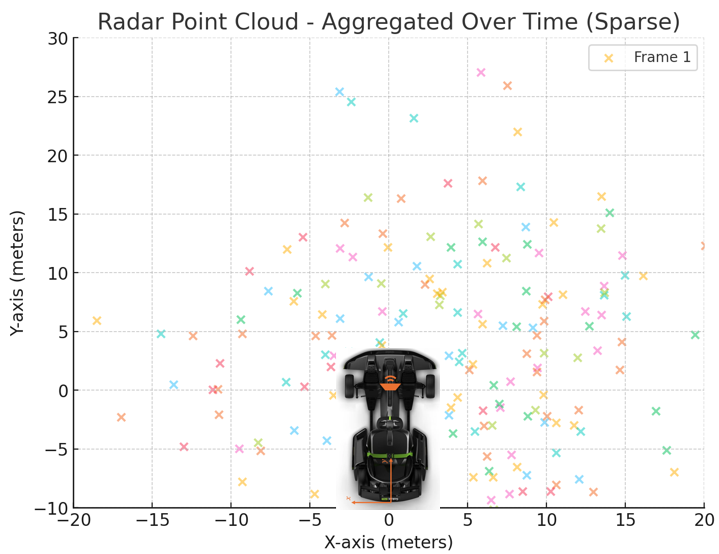
\includegraphics[width=0.5\linewidth]{images/multiframe.png}
    \caption{Frame Aggregation visualization.}
    \label{fig: Frame Aggregation visualization}
\end{figure}

This aggregation approach improves the accuracy of velocity and trajectory estimations, strengthens object identification's resilience against transient noise, and reduces problems related to sparse data.
It was implemented by using a stack with a fixed size, executing a "pop" operation prior to the insertion of the new frame at the stack's end.
The point cloud containing the points of all frames stored in the frame aggregator is then passed to the next stage.